\documentclass[11pt]{scrartcl}
\usepackage[T1]{fontenc}
\usepackage[a4paper, left=3cm, right=2cm, top=2cm, bottom=2cm]{geometry}
\usepackage[activate]{pdfcprot}
\usepackage[ngerman]{babel}
\usepackage[parfill]{parskip}
\usepackage[utf8]{inputenc}
\usepackage{kurier}
\usepackage{amsmath}
\usepackage{amssymb}
\usepackage{xcolor}
\usepackage{epstopdf}
\usepackage{txfonts}
\usepackage{fancyhdr}
\usepackage{graphicx}
\usepackage{prettyref}
\usepackage{hyperref}
\usepackage{eurosym}
\usepackage{setspace}
\usepackage{units}
\usepackage{eso-pic,graphicx}
\usepackage{icomma}
\usepackage{pdfpages}

\definecolor{darkblue}{rgb}{0,0,.5}
\hypersetup{pdftex=true, colorlinks=true, breaklinks=false, linkcolor=black, menucolor=black, pagecolor=black, urlcolor=darkblue}



\setlength{\columnsep}{2cm}


\newcommand{\arcsinh}{\mathrm{arcsinh}}
\newcommand{\asinh}{\mathrm{arcsinh}}
\newcommand{\ergebnis}{\textcolor{red}{\mathrm{Ergebnis}}}
\newcommand{\fehlt}{\textcolor{red}{Hier fehlen noch Inhalte.}}
\newcommand{\betanotice}{\textcolor{red}{Diese Aufgaben sind noch nicht in der Übung kontrolliert worden. Es sind lediglich meine Überlegungen und Lösungsansätze zu den Aufgaben. Es können Fehler enthalten sein!!! Das Dokument wird fortwährend aktualisiert und erst wenn das \textcolor{black}{beta} aus dem Dateinamen verschwindet ist es endgültig.}}
\newcommand{\half}{\frac{1}{2}}
\renewcommand{\d}{\, \mathrm d}
\newcommand{\punkte}{\textcolor{white}{xxxxx}}
\newcommand{\p}{\, \partial}
\newcommand{\dd}[1]{\item[#1] \hfill \\}

\renewcommand{\familydefault}{\sfdefault}
\renewcommand\thesection{}
\renewcommand\thesubsection{}
\renewcommand\thesubsubsection{}


\newcommand{\themodul}{Optische Technologie}
\newcommand{\thetutor}{Prof. Rateike}
\newcommand{\theuebung}{Übung 2}

\pagestyle{fancy}
\fancyhead[L]{\footnotesize{C. Hansen}}
\chead{\thepage}
\rhead{}
\lfoot{}
\cfoot{}
\rfoot{}

\title{\themodul{}, \theuebung{}, \thetutor}


\author{Christoph Hansen \\ {\small \href{mailto:chris@university-material.de}{chris@university-material.de}} }

\date{}


\begin{document}

\maketitle

Dieser Text ist unter dieser \href{http://creativecommons.org/licenses/by-nc-sa/4.0/}{Creative Commons} Lizenz veröffentlicht.

\textcolor{red}{Ich erhebe keinen Anspruch auf Vollständigkeit oder Richtigkeit. Falls ihr Fehler findet oder etwas fehlt, dann meldet euch bitte über den Emailkontakt.}

\tableofcontents


\newpage



\section{Aufgabe 1}


\begin{figure}[h]
	\centering
	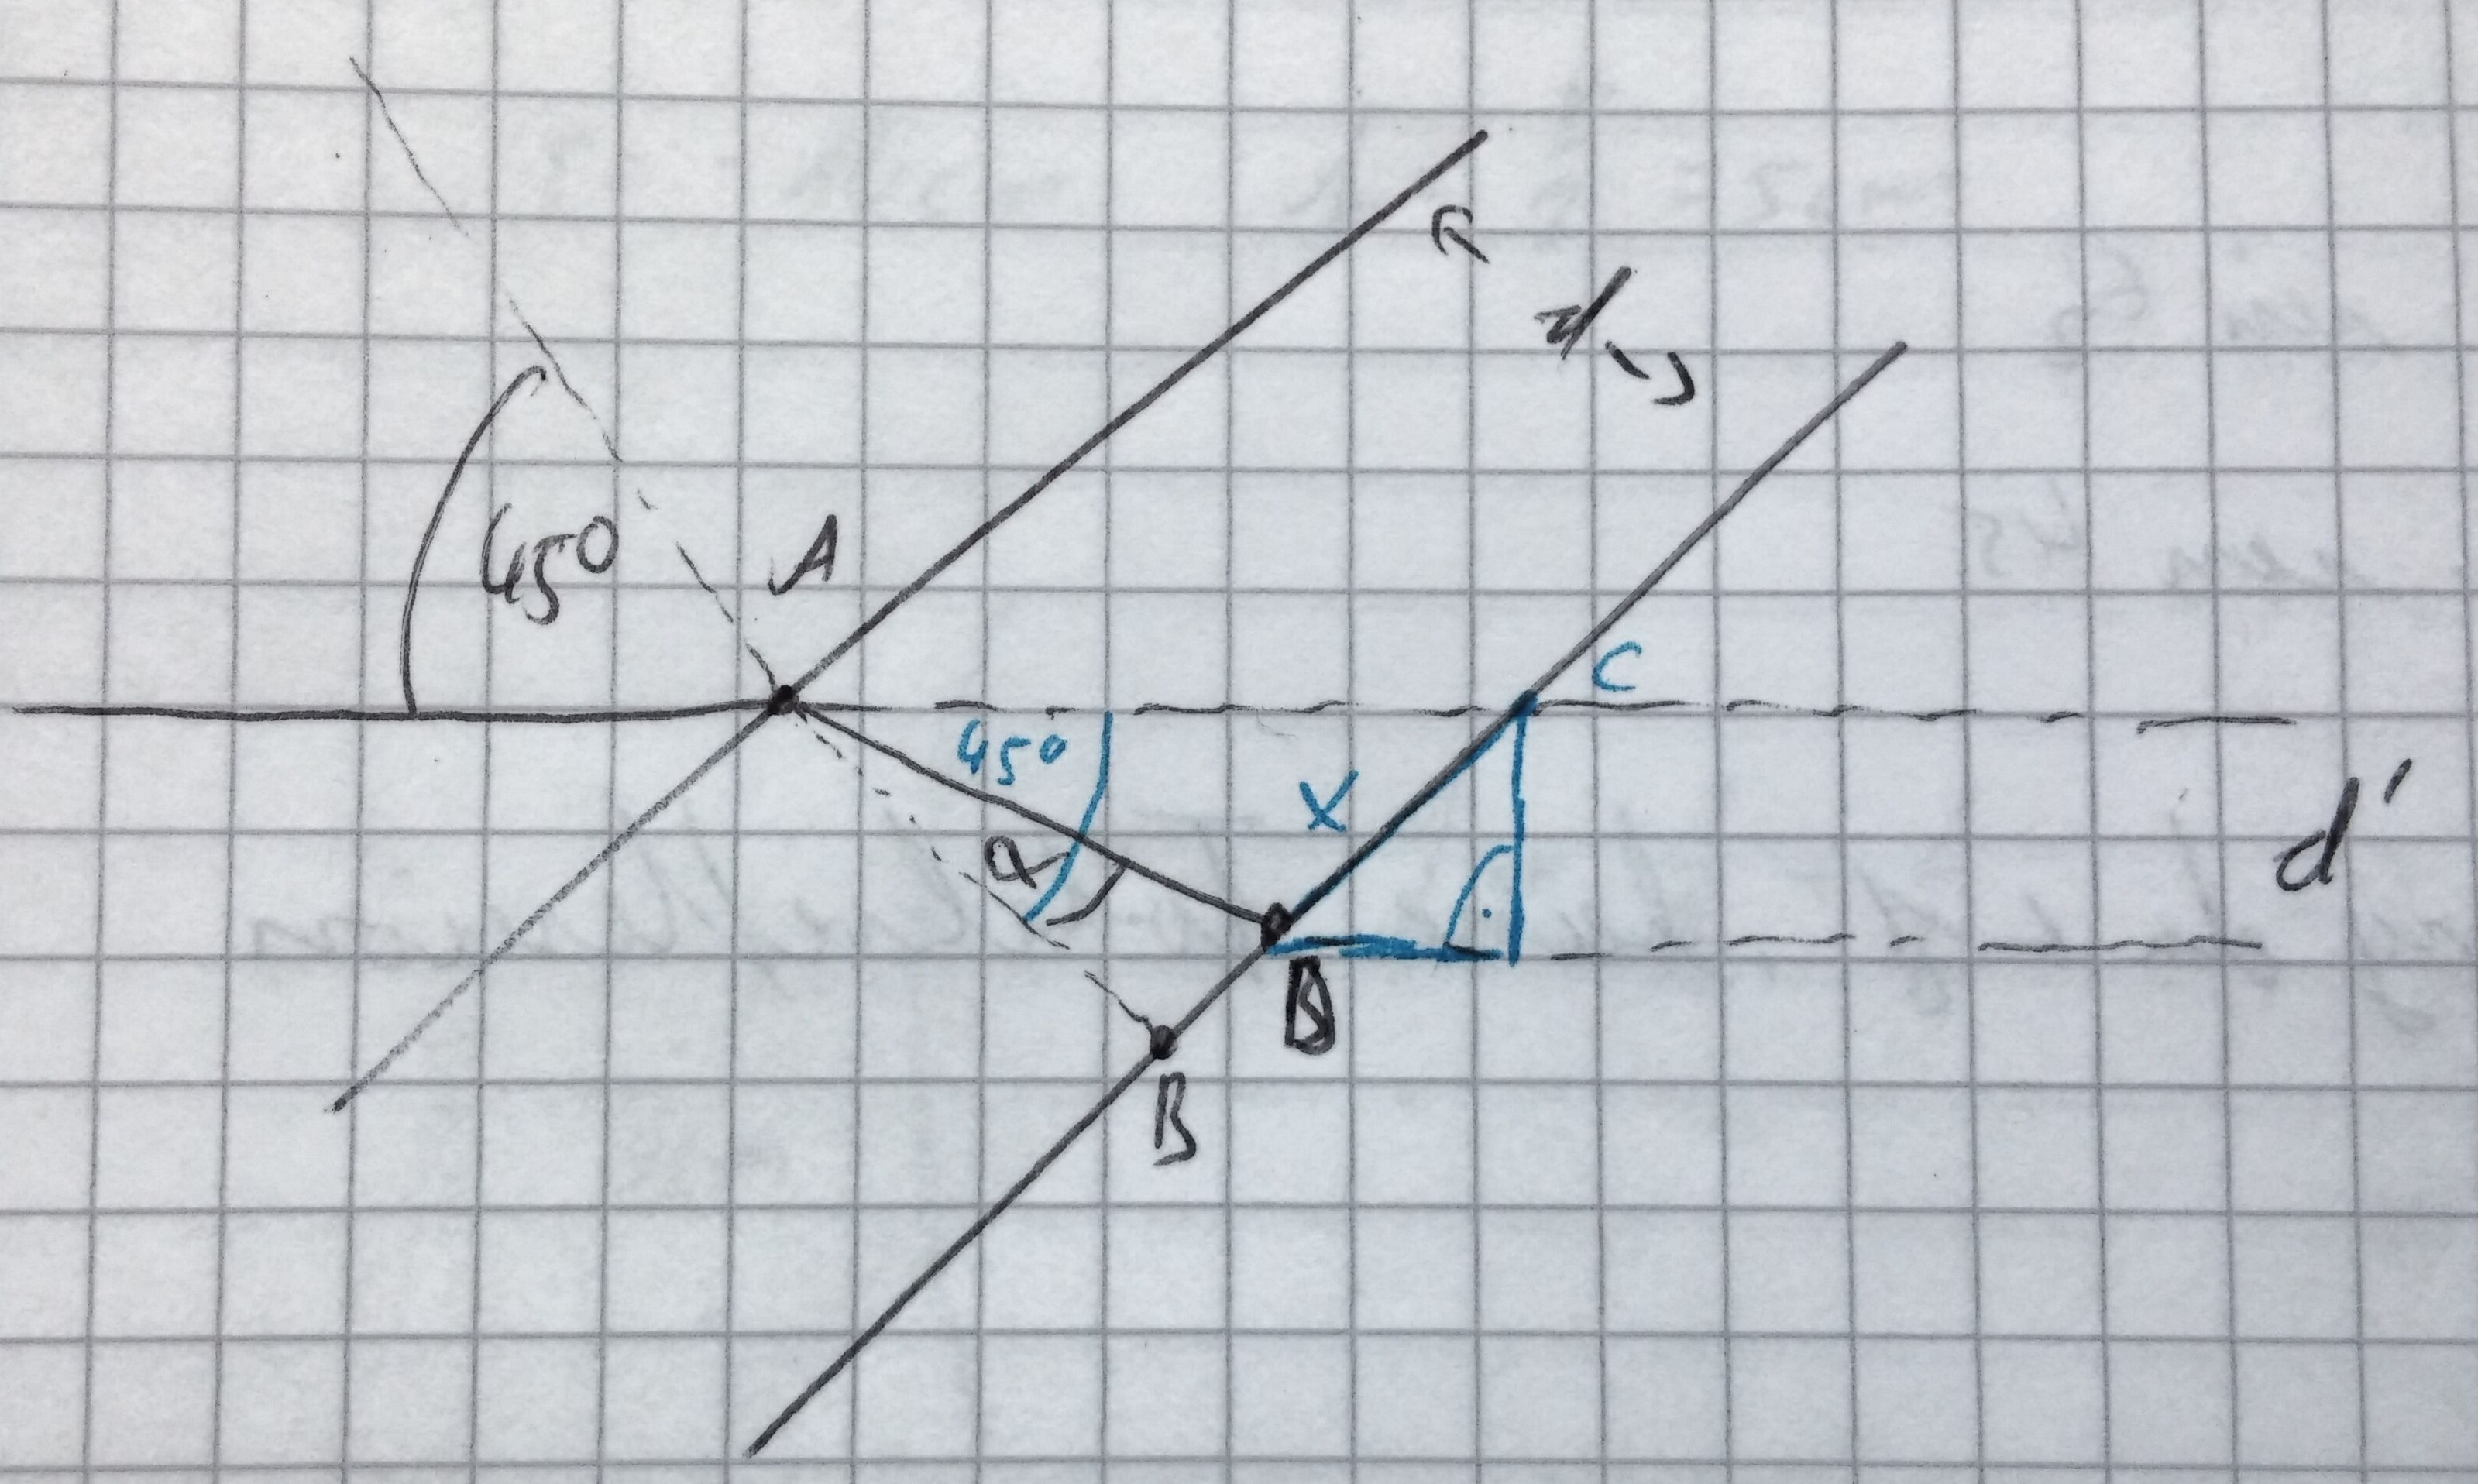
\includegraphics[scale=0.13]{A1_1.jpg}
\end{figure}


Wir rechnen mit Vielfachen des Radius R! Zunächst bestimmen wir die Geradengleichung für die dunkelblaue Gerade:

\begin{align*}
y_1 &= a \cdot x \qquad \text{mit} \qquad G = 0,1 \qquad \text{und} \qquad \overline{CG} = \frac{1}{3} \\
a &= \frac{G}{\overline{CG}} = \frac{0,1}{\frac{1}{3}} = 0,3 \\
\Rightarrow y_1 &= 0,3 \cdot x
\intertext{Nun stellen wir einen Zusammenhang zwischen $\alpha$ und $\beta$ her:}
n \cdot \sin(\alpha) &= \sin(\beta) \\
n \cdot \alpha &= \beta = \underbrace{1,5}_{Glas} \cdot \alpha
\intertext{Nun folgt die Gleichung für dir hellblaue Gerade. Mit der x-Achse schließt die Gerade den Winkel $\beta - \alpha$. Im weiteren ist $\beta - \alpha$ eine Steigung und kein Winkel!!}
\beta - \alpha &= 0,5 \cdot \alpha \\
\alpha &= \frac{G}{R} = \frac{0,1}{1} = 0,1 \\
\Rightarrow \beta - \alpha = 0,5 \cdot 0,1 = 0,05
\intertext{Wir schauen uns nun den Strahlengang an und stellen mit der Steigung und dem markanten Punkt P die Geradengleichung auf:}
y_2 &= 0,1 + 0,05 \cdot (x - 1) = 0,05x + 0,15
\intertext{Um den Schnittpunkt zu bestimmen, setzen wir beide Gleichungen gleich:}
y_1 &= y_2 \\
\Leftrightarrow 0,3x &= 0,05x - 0,15 \\
\Leftrightarrow 0,25x &= 0,15 \\
\Leftrightarrow x &= \frac{3}{5} = 0,6
\intertext{Über das Verhältnis von Bild zu Gegenstand berechnen wir die Bildgröße:}
\frac{B}{G} = \frac{0,6}{0,3} = 1,8
\end{align*}

Der Gegenstand wir also um den Faktor 1,8 vergrößert.


\section{Aufgabe 2}

\begin{align*}
\frac{1}{f} &= \left( 1,52 - 1 \right) \cdot \left( \frac{1}{50} - \frac{1}{-50} \right) = \frac{0,52}{25} \\
\Leftrightarrow f &= \frac{25}{0,52} = \unit[48,1]{mm}
\end{align*}


\section{Aufgabe 3}

\begin{align*}
\frac{1}{f} &= \left( 1,52 - 1 \right) \cdot \left( \frac{1}{100} - \frac{1}{-\infty} \right) = \frac{0,52}{100} \\
\Leftrightarrow f &= \frac{100}{0,52} = \unit[192,3]{mm}
\end{align*}


\section{Aufgabe 4}

\begin{figure}[h]
	\centering
	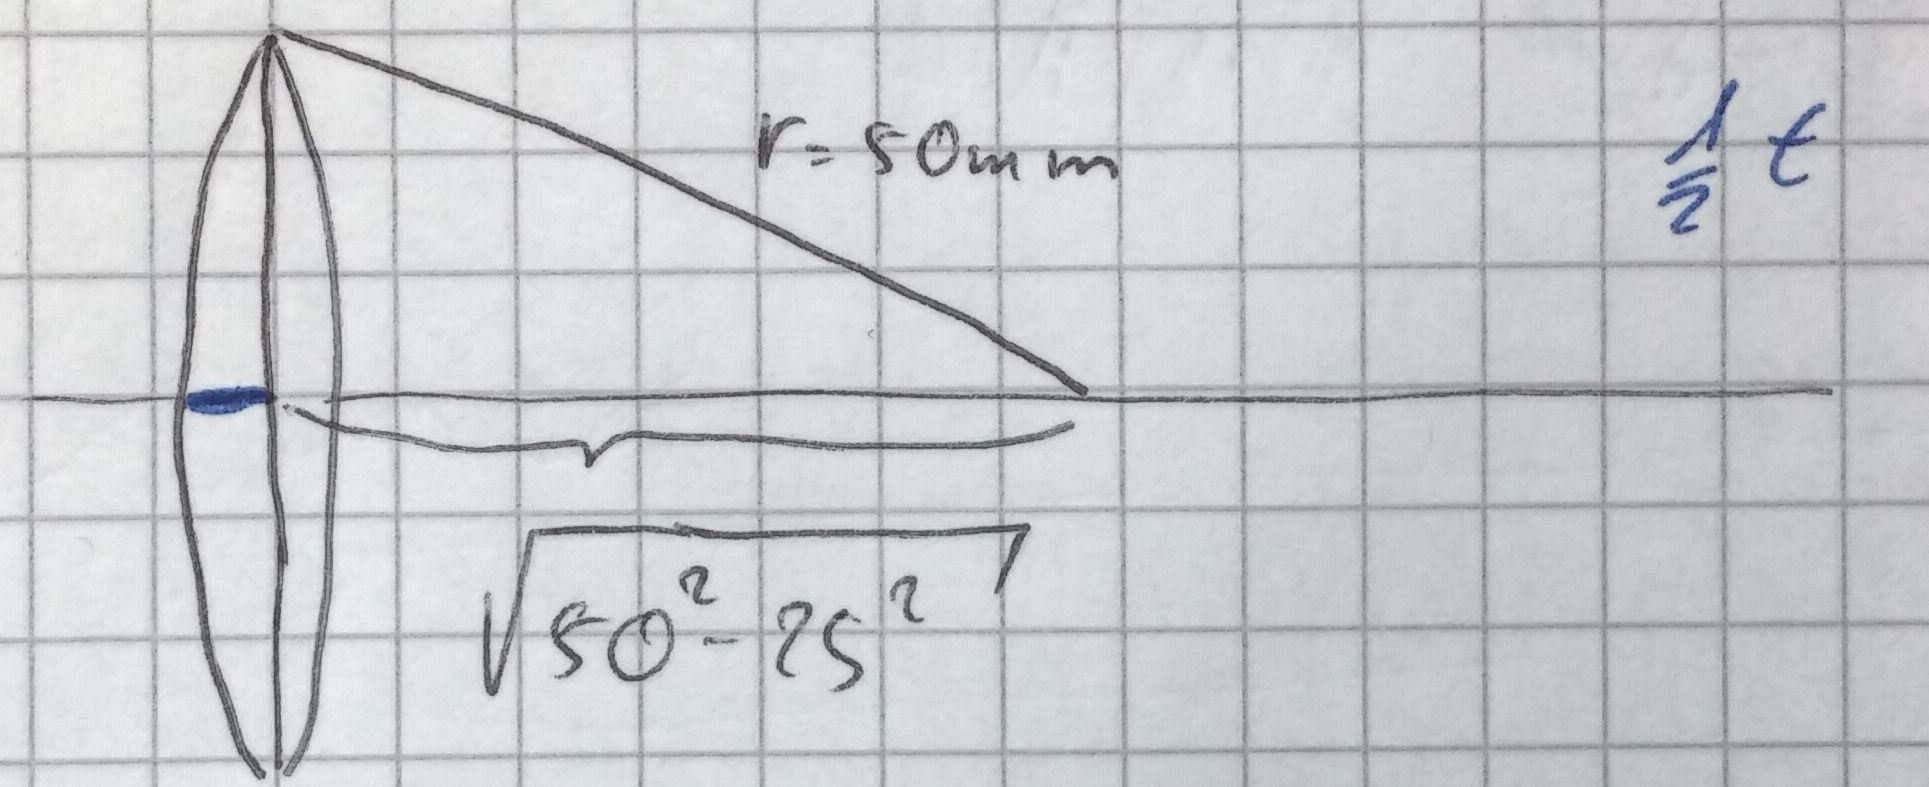
\includegraphics[scale=0.16]{A4_1.jpg}
\end{figure}


Für die blaue Strecke $\half t$ gilt:

\begin{align*}
\half t &= 50 - \sqrt{50^2 - 25^2} \\
\Leftrightarrow t &= \unit[13,4]{mm}
\intertext{Dies können wir in die Gleichung für dicke Linsen einsetzen:}
\frac{1}{f} &= \left( 1,52 - 1 \right) \cdot \left( \frac{1}{50} - \frac{1}{-50} + \frac{0,52 \cdot 13,4}{1,52 \cdot 50 \cdot -50} \right) \\
\Leftrightarrow f &= \unit[50,4]{mm}
\end{align*}


\section{Aufgabe 5}

Bei einer planen Fläche auf einer Seite, wird einer der Radien $\infty$ und damit wird der Korrekturterm der dicken Linse $0$ und fällt weg und wir erhalten die selbe Brennweite wie in Aufgabe 2.

\end{document}